\documentclass[12pt]{article}
\usepackage[utf8]{inputenc}
\usepackage{graphicx} % Allows you to insert figures
\usepackage{subcaption}
\usepackage{amsmath} % Allows you to do equations
\usepackage{fancyhdr} % Formats the header
\usepackage{geometry} % Formats the paper size, orientation, and margins
\usepackage{dirtytalk} % typesetting different types of quotation
\usepackage[english]{babel}
\usepackage{csquotes}
\usepackage{hyperref}
\usepackage{listings}
\lstset{
    language=C,
    basicstyle=\ttfamily, 
    numberstyle=\tiny,
    frame=single,
    breaklines=true,
}

\linespread{1.25} % About 1.5 spacing in Word
\setlength{\parindent}{0.8cm} % No paragraph indents
\setlength{\parskip}{0em} % Paragraphs separated by one line
\renewcommand{\headrulewidth}{0pt} % Removes line in header
\geometry{a4paper, portrait, margin=1in}
\setlength{\headheight}{14.49998pt}
\graphicspath{ {images/} }

\begin{document}
\begin{titlepage}
   \begin{center}
    \textsc{\large Ministry of Education of Republic of Moldova}\\[0.5cm]
    \textsc{\large Technical University of Moldova}\\[0.5cm]
    \textsc{\large Faculty of Computers, Informatics and Microelectronics}\\[0.5cm]
    \textsc{\large Software Engineering Department}\\[1.2cm]
    
    \vspace{25 mm}
    
    \textsc{\Large Computer Programming}\\[0.5cm]
    \textsc{\large Laboratory work \#3}\\[0.5cm]    % <<<<<<< CHANGE LAB NUMBER HERE
    
    \newcommand{\HRule}{\rule{\linewidth}{0.5mm}}
    \vspace{10 mm}
    \HRule \\[0.4cm]
    { \LARGE \bfseries Two-Dimensional Array Operations and Processing }\\[0.4cm] % <<<<<<< CHANGE LAB TITLE HERE
    \HRule \\[1.5cm]
    
    \vspace{10mm}
    
    \begin{minipage}[t]{0.4\textwidth}
    \begin{flushleft} \large
    \emph{Author:} \\
    Mihai \textsc{Caraman}\\                         % <<<<<<< CHANGE YOUR NAME HERE
    std. gr. FAF-233                                % <<<<<<< CHANGE GROUP NUMBER HERE
    \end{flushleft}
    \end{minipage}
    ~
    \begin{minipage}[t]{0.4\textwidth}
    \begin{flushright} \large
    \emph{Verified:} \\
    Alexandru \textsc{Furdui}\\
    \end{flushright}
    \end{minipage}\\[3cm]
    
    \vspace{5 mm}
    \large Chișinău 2023\\[0.5cm]
    
    \vfill
    \end{center}
\end{titlepage}

\setcounter{page}{2}
\pagestyle{fancy}
\fancyhf{}
\rhead{\thepage}
\lhead{FAF-233 Mihai Caraman; Laboratory Work №3}

% \section*{Introduction}
\section*{Theory Background}
\hspace{0.8cm}A two-dimensional array is a data structure that organizes data in a grid-like format, consisting of rows and columns. Each element in a 2D array is identified by two indices: a row index and a column index.
Two-dimensional arrays are fundamental in programming and are used for various applications, including representing images, matrices, grids, game boards, and more. Understanding their operations and processing is crucial for efficient manipulation and utilization of structured data.

\section*{The Task}

Describe your task, and enumerate the task/tasks you have implemented:
\begin{enumerate}
  \item Task: Hard - Constructing a Mountain Matrix(worth 10 points)
\end{enumerate}


\section*{Technical implementation}
Pseudocode
\begin{lstlisting}
Define function InsertionSort(array, length)
    For i = 1 to length - 1
        Set key = array[i]
        Set j = i - 1
        While j >= 0 and array[j] > key
            Move array[j] to array[j + 1]
            Set j = j - 1
        End While
        Set array[j + 1] = key
    End For
End Function

Define function printSpiral(rows, cols, matrix, array)
    Set top = 0, bottom = rows - 1, left = 0, right = cols - 1
    Set index = 0
    While top <= bottom and left <= right
        For i = left to right
            Set matrix[top][i] = array[index++]
        End For
        Increment top

        For i = top to bottom
            Set matrix[i][right] = array[index++]
        End For
        Decrement right

        If top <= bottom
            For i = right to left
                Set matrix[bottom][i] = array[index++]
            End For
            Decrement bottom
        End If
        
        If left <= right
            For i = bottom to top
                Set matrix[i][left] = array[index++]
            End For
            Increment left
        End If
    End While
End Function

Define function main()
    Read rows from user
    Read cols from user
    Create 2D matrix with dimensions rows and cols
    For i = 0 to rows - 1
        For j = 0 to cols - 1
            Read matrix[i][j] from user
        End For
    End For
    Convert 2D matrix to 1D array
    Call InsertionSort with array and length
    Print sorted 2D array in a matrix-like format
    Call printSpiral with rows, cols, matrix, and array
    Print matrix in a clockwise spiral pattern
End Function

\end{lstlisting}

\section*{Results}
\hspace{0.8cm} The program takes user input for the number of rows and columns, followed by input for the elements of a matrix. It then performs the following operations:

\paragraph{Insertion Sort:}
\begin{itemize}
  \item Converts the 2D matrix into a 1D array.
  \item Sorts the 1D array using the Insertion Sort algorithm.
\end{itemize}

\paragraph{Print Sorted 2D Array as a Matrix:}
\begin{itemize}
    \item Prints the sorted 1D array as a matrix, using the specified number of columns.
\end{itemize}

\paragraph{Print Matrix in a Clockwise Spiral Pattern:}
\begin{itemize}
    \item Calls a function (printSpiral) to fill and print the matrix in a clockwise spiral pattern.
\end{itemize}

\paragraph{User Input:}
\begin{itemize}
    \item User provides the number of rows (e.g., 3) and columns (e.g., 4).
    \item User inputs elements for a 3x4 matrix.
\end{itemize}

\paragraph{Insertion Sort and 1D Array Conversion:}
\begin{itemize}
    \item The program converts the 2D matrix to a 1D array, which is then sorted using Insertion Sort.
\end{itemize}

\paragraph{Print Sorted 2D Array as a Matrix:}
\begin{itemize}
    \item The program prints the sorted 1D array in a matrix-like format using the specified number of columns.
\end{itemize}

\paragraph{Print Matrix in a Clockwise Spiral Pattern:}
\begin{itemize}
    \item The program fills and prints the original matrix in a clockwise spiral pattern using the sorted array.
\end{itemize}

\paragraph{Output:}
\begin{itemize}
    \item The sorted 1D array is printed in a matrix-like format.
    \item The original matrix is printed in a clockwise spiral pattern.
\end{itemize}

The actual output, such as the sorted 1D array and the matrix in a clockwise spiral pattern, will depend on the specific input provided by the user. The program demonstrates the sorting of a 1D array, conversion of a 2D matrix to a 1D array, and a visualization of the original matrix in a spiral pattern.


\begin{figure}
    \centering
    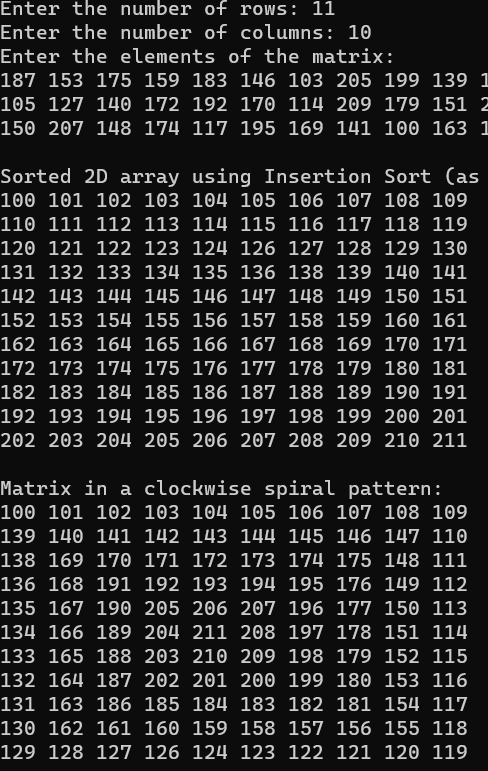
\includegraphics[width=0.75\linewidth]{Screenshot 2023-10-06 212655.png}
    \caption{The results from the console}
    \label{fig:enter-label}
\end{figure}
           
\section*{Conclusion}
\hspace{0.8cm}
Functionality: Code performs sorting using Insertion Sort on a 1D array obtained from a 2D matrix. It visualizes the sorted array as a matrix and displays the original matrix in a clockwise spiral pattern.

Input Processing: Accepts user input for matrix dimensions and elements, demonstrating user interaction.

Modular Design: Well-structured code with separate functions for sorting and matrix traversal, promoting code reuse and readability.

Visualization: Effectively displays the sorted array in a matrix-like format and visualizes the original matrix in a clockwise spiral pattern.

Optimization Potential: Room for optimization, especially in memory usage and code readability.

User Interaction and Feedback: Provides clear prompts for user input, enhancing user understanding and interaction.


\section*{Bibliography}
\hspace{0.8cm}
\begin{enumerate}
  \item https://stackoverflow.com/
  \item https://www.geeksforgeeks.org/
  \item https://github.com/caramisca/Lab-3  (github link with all docs, source code, pdf file, .tex file)
\end{enumerate}

\pagebreak
\end{document}